\chapter{Vector fields} \label{s:vec}

\minitoc

\section{Introduction}

This chapter is devoted to the most basic objects of tensor calculus:
vector fields. We start by defining tangent vectors and tangent spaces
on a differentiable manifold (Sec.~\ref{s:vec:tangent_vectors}), and then
move to vector fields (Sec.~\ref{s:vec:vector_fields}).

\section{Tangent vectors} \label{s:vec:tangent_vectors}

\subsection{Definitions} \label{s:vec:def_tangent_vector}

Let $\M$ be a smooth manifold of dimension $n$ over the topological field $\K$
and $C^\infty(M)$ the corresponding algebra of scalar fields introduced in Sec.~\ref{s:man:scal_algebra}.
For $p\in M$, a \defin{tangent vector at}\index{tangent!vector} $p$ is
a map
\be
    \w{v}: C^\infty(M) \longrightarrow \K
\ee
such that (i) $\w{v}$ is $\K$-linear and (ii) $\w{v}$ obeys
\be \label{e:vec:derivation}
    \forall f,g \in C^\infty(M),\quad
        \w{v}(fg) = \w{v}(f) g(p) + f(p) \w{v}(g) .
\ee
Because of property~\eqref{e:vec:derivation}, one says that $\w{v}$ is
a \defin{derivation at} $p$.

The set $T_p\M$ of all tangent vectors at $p$ is a vector space of dimension
$n$ over $\K$; it is called the \defin{tangent space to} $\M$
\defin{at}\index{tangent!space} $p$.

\subsection{SageMath implementation} \label{s:vec:tangent_impl}

To illustrate the implementation of tangent vectors in \Sage{}, we shall
consider the same example $M=\Sp$ as in Chap.~\ref{s:man}. First of all,
we recreate the same objects as in Chap.~\ref{s:man}, starting with the manifold
$M$ and its two stereographic charts $X_U = (U,(x,y))$ and $X_V = (V,(x',y'))$,
with $M=U\cup V$ (the full Jupyter notebook is available at
\url{https://sagemanifolds.obspm.fr/jncf2018/}):
\setcounter{NBin}{0}
\begin{NBin}
%display latex
\end{NBin}
\begin{NBin}
M = Manifold(2, 'M')
U = M.open_subset('U')
XU.<x,y> = U.chart()
V = M.open_subset('V')
XV.<xp,yp> = V.chart("xp:x' yp:y'")
M.declare_union(U,V)
XU_to_XV = XU.transition_map(XV,
                             (x/(x^2+y^2), y/(x^2+y^2)),
                             intersection_name='W',
                             restrictions1= x^2+y^2!=0,
                             restrictions2= xp^2+yp^2!=0)
XV_to_XU = XU_to_XV.inverse()
M.atlas()
\end{NBin}
\begin{NBoutM}
\left[\left(U,(x, y)\right), \left(V,({x'}, {y'})\right), \left(W,(x, y)\right), \left(W,({x'}, {y'})\right)\right]
\end{NBoutM}
Then we introduce the point $p\in U$ of coordinates $(x,y)=(1,2)$:
\begin{NBin}
p = U((1,2), chart=XU, name='p')
print(p)
\end{NBin}
\begin{NBprint}
Point p on the 2-dimensional differentiable manifold M
\end{NBprint}
The canonical embedding of $\Sp$ in $\R^3$ is defined mostly for
graphical purposes:
\begin{NBin}
R3 = Manifold(3, 'R^3', r'\mathbb{R}^3')
XR3.<X,Y,Z> = R3.chart()
Phi = M.diff_map(R3, {(XU, XR3):
                       [2*x/(1+x^2+y^2), 2*y/(1+x^2+y^2),
                       (x^2+y^2-1)/(1+x^2+y^2)],
                      (XV, XR3):
                       [2*xp/(1+xp^2+yp^2), 2*yp/(1+xp^2+yp^2),
                       (1-xp^2-yp^2)/(1+xp^2+yp^2)]},
                  name='Phi', latex_name=r'\Phi')
Phi.display()
\end{NBin}
\begin{NBoutM}
\begin{array}{llcl} \Phi:& M & \longrightarrow & \mathbb{R}^3 \\ \mbox{on}\ U : & \left(x, y\right) & \longmapsto & \left(X, Y, Z\right) = \left(\frac{2 \, x}{x^{2} + y^{2} + 1}, \frac{2 \, y}{x^{2} + y^{2} + 1}, \frac{x^{2} + y^{2} - 1}{x^{2} + y^{2} + 1}\right) \\ \mbox{on}\ V : & \left({x'}, {y'}\right) & \longmapsto & \left(X, Y, Z\right) = \left(\frac{2 \, {x'}}{{x'}^{2} + {y'}^{2} + 1}, \frac{2 \, {y'}}{{x'}^{2} + {y'}^{2} + 1}, -\frac{{x'}^{2} + {y'}^{2} - 1}{{x'}^{2} + {y'}^{2} + 1}\right) \end{array}
\end{NBoutM}
\vspace*{-\baselineskip}
\begin{NBin}
graph = XU.plot(chart=XR3, mapping=Phi, number_values=25,
                label_axes=False) + \
        XV.plot(chart=XR3, mapping=Phi, number_values=25,
                color='green', label_axes=False) + \
        p.plot(chart=XR3, mapping=Phi, label_offset=0.05)
show(graph, viewer='threejs', online=True)
\end{NBin}
\begin{center}
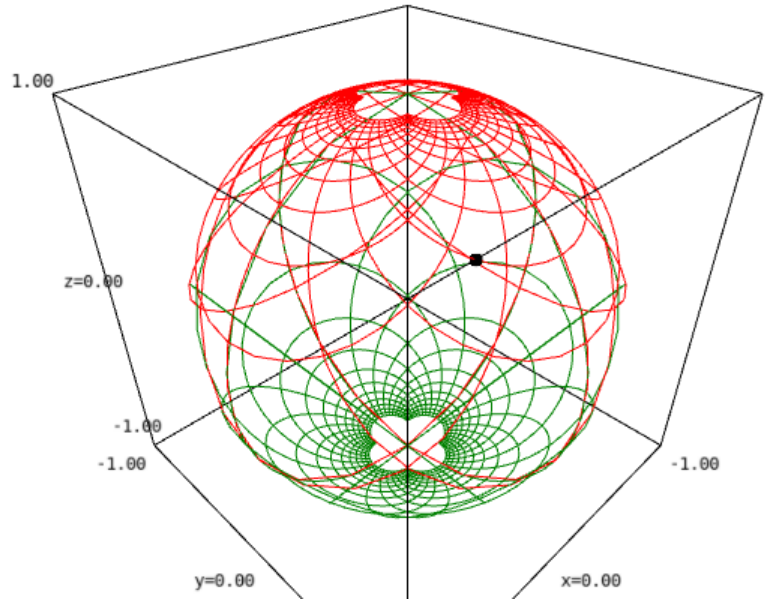
\includegraphics[width=0.8\textwidth]{sphere_stereo.png}
\end{center}
Finally, the last objects defined in Chap.~\ref{s:man} are the
scalar field $f$:
\begin{NBin}
f = M.scalar_field({XU: 1/(1+x^2+y^2), XV: (xp^2+yp^2)/(1+xp^2+yp^2)},
                   name='f')
f.display()
\end{NBin}
\begin{NBoutM}
\begin{array}{llcl} f:& M & \longrightarrow & \mathbb{R} \\ \mbox{on}\ U : & \left(x, y\right) & \longmapsto & \frac{1}{x^{2} + y^{2} + 1} \\ \mbox{on}\ V : & \left({x'}, {y'}\right) & \longmapsto & \frac{{x'}^{2} + {y'}^{2}}{{x'}^{2} + {y'}^{2} + 1} \end{array}
\end{NBoutM}
and its parent, namely the commutative algebra $C^\infty(\M)$ of
smooth maps $\M\to\R$:
\begin{NBin}
CM = M.scalar_field_algebra()
CM
\end{NBin}
\begin{NBoutM}
C^{\infty}\left(M\right)
\end{NBoutM}

The tangent space at the point $p$ introduced in \code{In~[3]} is generated by
\begin{NBin}
Tp = M.tangent_space(p)
Tp
\end{NBin}
\begin{NBoutM}
T_{p}\,M
\end{NBoutM}
It is a vector space over $\K$ (here $\K=\R$, which is represented by \Sage{}'s Symbolic
Ring \code{SR}):
\begin{NBin}
print(Tp.category())
\end{NBin}
\begin{NBprint}
Category of finite dimensional vector spaces over Symbolic Ring
\end{NBprint}
The dimension of the vector space $T_p\M$ equals that of the manifold $\M$:
\begin{NBin}
dim(Tp)
\end{NBin}
\begin{NBoutM}
2
\end{NBoutM}
Tangent spaces are implemented as a class inherited from \code{TangentSpace}
via the category framework:
\begin{NBin}
type(Tp)
\end{NBin}
\begin{NBout}
\begin{verbatim}
<class
 'sage.manifolds.differentiable.tangent_space.TangentSpace_with_category'>
\end{verbatim}
\end{NBout}
\code{FiniteRankFreeModule},\footurl{http://doc.sagemath.org/html/en/reference/tensor_free_modules/sage/tensor/modules/finite_rank_free_module.html}, which, in \Sage{} is devoted to free modules of finite rank
without any distinguished basis:
\begin{NBin}
isinstance(Tp, FiniteRankFreeModule)
\end{NBin}
\begin{NBout}
\texttt{True}
\end{NBout}
\begin{remark}
In \Sage{}, free modules with a distinguished basis
are created with the command \code{FreeModule} or \code{VectorSpace}
and belong to classes different from \code{FiniteRankFreeModule}.
The differences are illustrated at\\
{\scriptsize \url{http://doc.sagemath.org/html/en/reference/modules/sage/tensor/modules/finite_rank_free_module.html#diff-freemodule}}.
\end{remark}

Two bases of $T_p\M$ are already available: those generated by the derivations
at $p$ along the coordinates of charts \code{XU} and \code{XV} respectively:
\begin{NBin}
Tp.bases()
\end{NBin}
\begin{NBoutM}
\left[\left(\frac{\partial}{\partial x },\frac{\partial}{\partial y }\right), \left(\frac{\partial}{\partial {x'} },\frac{\partial}{\partial {y'} }\right)\right]
\end{NBoutM}
None of these bases is distinguished, but one if the default one, which
simply means that it is the basis to be considered if the basis argument
is skipped in some methods:
\begin{NBin}
Tp.default_basis()
\end{NBin}
\begin{NBoutM}
\left(\frac{\partial}{\partial x },\frac{\partial}{\partial y }\right)
\end{NBoutM}

A tangent vector is created as an element of the tangent space by the
standard \Sage{} procedure\index{parent}\index{element}
\code{new\_element = parent(...)}, where \code{...}
stands for some material sufficient to construct the element:
\begin{NBin}
vp = Tp((-3, 2), name='v')
print(vp)
\end{NBin}
\begin{NBprint}
Tangent vector v at Point p on the 2-dimensional differentiable manifold M
\end{NBprint}
Since the basis is not specified, the pair $(-3,2)$ refers to components
with respect to the default basis:
\begin{NBin}
vp.display()
\end{NBin}
\begin{NBoutM}
v = -3 \frac{\partial}{\partial x } + 2 \frac{\partial}{\partial y }
\end{NBoutM}
We have of course
\begin{NBin}
vp.parent()
\end{NBin}
\begin{NBoutM}
T_{p}\,M
\end{NBoutM}
\vspace*{-\baselineskip}
\begin{NBin}
vp in Tp
\end{NBin}
\begin{NBout}
\texttt{True}
\end{NBout}
As other manifold objects, tangent vectors have some plotting capabilities:
\begin{NBin}
graph += vp.plot(chart=XR3, mapping=Phi, scale=0.5, color='gold')
show(graph, viewer='threejs', online=True)
\end{NBin}
\begin{NBout}
\emph{(see Figure~\ref{out2})}
\end{NBout}
\begin{figure}
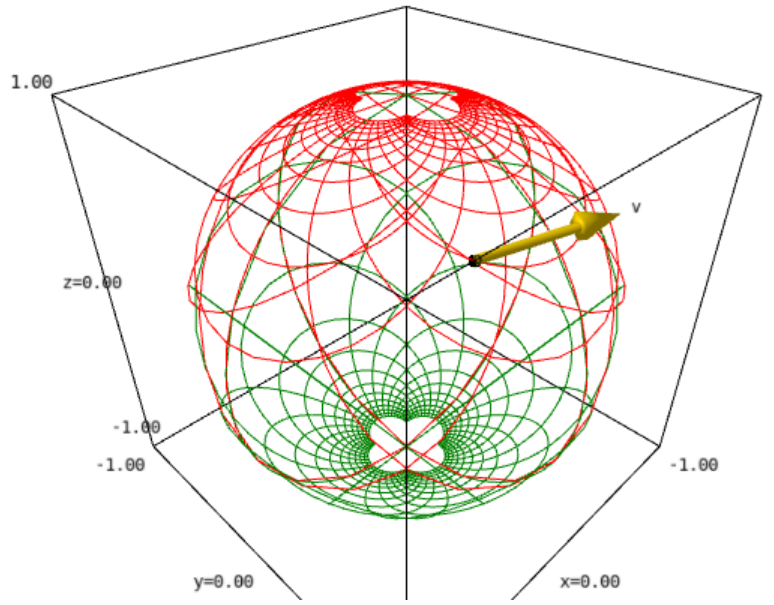
\includegraphics[width=0.8\textwidth]{sphere_tan_vect.png}
\caption{Output corresponding to \texttt{In [\theNBin]}.}\label{out2}
\end{figure}

The main attribute of the object \code{vp} representing the vector $\w{v}$ is the
private dictionary \code{\_components}, which stores the components of $\w{v}$ in various bases of $T_p M$:
\begin{NBin}
vp._components
\end{NBin}
\begin{NBout}
$\displaystyle
\bigg\{\left(\frac{\partial}{\partial x },\frac{\partial}{\partial y }\right) :$\\
\texttt{1-index components w.r.t.~Basis (d/dx,d/dy) on the Tangent space at Point p on the 2-dimensional differentiable manifold M}
$\bigg\}$
\end{NBout}
The keys of the dictionary \code{\_components} are the bases of $T_p M$, while the values belong to the class \code{Components}\footurl{http://doc.sagemath.org/html/en/reference/tensor_free_modules/sage/tensor/modules/comp.html} devoted to store ring elements indexed by integers or tuples of integers:
\begin{NBin}
vpc = vp._components[Tp.default_basis()]
vpc
\end{NBin}
\begin{NBout}
\texttt{1-index components w.r.t.~Basis (d/dx,d/dy) on the Tangent space at Point p
on the 2-dimensional differentiable manifold M}
\end{NBout}
\vspace*{-\baselineskip}
\begin{NBin}
type(vpc)
\end{NBin}
\begin{NBout}
\begin{verbatim}
<class 'sage.tensor.modules.comp.Components'>
\end{verbatim}
\end{NBout}
The components themselves are stored in the private dictionary \code{\_comp} of the \code{Components} object, with the indices as keys:
\begin{NBin}
vpc._comp
\end{NBin}
\begin{NBoutM}
\left\{\left(0\right) : -3, \left(1\right) : 2\right\}
\end{NBoutM}
Hence the components are not stored via a sequence data type (list or tuple), as
one might have expected, but via a mapping type (dictionary). This is a general
feature of the class \code{Components} and all its subclasses, which permits
to not store vanishing components and, in case of symmetries (for multi-index
objects like tensors), to store only non-redundant components.

%%%%%%%%%%%%%%%%%%%%%%%%%%%%%%%%%%%%%%%%%%%%%%%%%%%%%%%%%%%%%%%%%%%%%%%%%%%%%%%

\section{Vector fields} \label{s:vec:vector_fields}

\subsection{Definition}

The \defin{tangent bundle}\index{tangent!bundle} of $\M$ is the disjoint union
of the tangent spaces at all points of $\M$:
\be
    T\M = \coprod_{p\in\M} T_p \M .
\ee
Elements of $T\M$ are usually denoted by $(p, \w{u})$, with $\w{u}\in T_p\M$.
The tangent bundle is canonically endowed with the
\defin{projection map}\index{projection!map}:
\be
    \begin{array}{cccc}
    \pi : & T\M & \longrightarrow & \M \\
        & (p,\w{u}) & \longmapsto & p .
    \end{array}
\ee

The tangent bundle inherits some manifold structure from $\M$:
$T\M$ is a smooth manifold of dimension $2n$ over $\K$ ($n$ being the dimension
of $\M$).

A \defin{vector field}\index{vector!field} on $\M$ is a continuous
right-inverse of the projection map, i.e.\ it is a map
\be
    \begin{array}{cccc}
    \w{v} : & \M & \longrightarrow & T\M \\
        & p & \longmapsto & \left. \w{v}\right| _p
    \end{array}
\ee
such that $\pi\circ \w{v} = \mathrm{Id}_{\M}$, i.e.\ such that
\be
    \forall p\in \M, \quad \left. \w{v}\right| _p \in T_p\M .
\ee

\subsection{Module of vector fields} \label{s:vec:vector_module}

The set $\X(\M)$ of all vector fields on $\M$
is naturally endowed with two algebraic structures:
\begin{enumerate}
\item $\X(\M)$ is a (infinite dimensional) vector space over $\K$ --- the base field of $\M$ ---,
the scalar multiplication $\K\times\X(M)\to \X(M)$, $(\lambda,\w{v})\mapsto \lambda \w{v}$
being defined by
\be
    \forall p\in\M,
    \quad \left. (\lambda \w{v}) \right| _p =  \left. \lambda \w{v} \right| _p,
\ee
where
the right-hand side involves the scalar multiplication
in the vector space $T_p\M$;
\item $\X(\M)$ is a module\index{module} over $C^\infty(M)$ --- the commutative
algebra of scalar fields ---,
the scalar multiplication $C^\infty(M)\times\X(M)\to \X(M)$, $(f,\w{v})\mapsto f \w{v}$
being defined by
\be
    \forall p\in\M,
    \quad \left. (f \w{v}) \right| _p = \left.f(p)  \w{v} \right| _p ,
\ee
where
the right-hand side involves the scalar multiplication by $f(p)\in \K$
in the vector space $T_p\M$.
\end{enumerate}
An important subcase of 2 is when $\X(\M)$ is a
\defin{free module}\index{free module}\index{module!free --} over $C^\infty(M)$,
i.e.\ when $\X(\M)$ admits a basis\index{basis} (a generating set consisting of linearly independent elements). If this occurs, then $\X(\M)$ is actually a
\defin{free module of finite rank}\index{free module!of finite rank}\index{finite rank!free module of --} over $C^\infty(M)$ and its rank is $n$ -- the dimension of
$\M$ over $\K$, which means that all bases share the same cardinality, namely $n$.
One says that $\M$ is a \defin{parallelizable}\index{parallelizable} manifold.
A basis $(\w{e}_a)_{1\leq a \leq n}$ of $\X(\M)$ is called a
\defin{vector frame}\index{vector!frame};
for any $p\in\M$, $(\left.\w{e}_a \right| _p)_{1\leq a \leq n}$
is then a basis of the tangent vector space $T_p\M$.
Any vector field has a unique decomposition with respect to the vector
frame\footnote{Einstein's convention for summation on repeated indices is assumed.} $(\w{e}_a)_{1\leq a \leq n}$:
\be \label{e:vec:v_expand}
    \forall \w{v}\in\X(\M),\quad \w{v} = v^a \w{e}_a,\quad\mbox{with\ } v^a \in C^\infty(\M) .
\ee
At each point $p\in \M$, Eq.~\eqref{e:vec:v_expand} gives birth to an identity in
the tangent space $T_p \M$:
\be
    \left.\w{v} \right| _p = v^a(p)  \left.\w{e}_a \right| _p,\quad\mbox{with\ } v^a(p) \in \K ,
\ee
which is nothing but the expansion of the tangent vector $\left.\w{v} \right| _p$
on the basis $(\left.\w{e}_a \right| _p)_{1\leq a \leq n}$ of the
vector space $T_p \M$.

Note that if $\M$ is covered by a chart $X$, i.e.~$\M$ is the domain of
the chart $X$, then $\M$ is parallelizable and a vector frame
is $(\partial/\partial x^a)_{1\leq a \leq n}$, where the $x^a$'s are
the coordinates of chart $X$. Such a vector frame is called a
\defin{coordinate frame}\index{coordinate!frame} or \defin{natural basis}\index{natural basis}. More generally, examples of parallelizable manifolds are
\cite{Lee13}
\begin{itemize}
\item the Cartesian space $\mathbb{R}^n$ for $n=1,2,\ldots$,
\item the circle $\mathbb{S}^1$,
\item the torus $\mathbb{T}^2 = \mathbb{S}^1\times \mathbb{S}^1$,
\item the sphere $\mathbb{S}^3 \simeq \mathrm{SU}(2)$, as any Lie group,
\item the sphere $\mathbb{S}^7$,
\item any orientable 3-manifold (Steenrod theorem~\cite{Steen51}).
\end{itemize}
On the other hand, examples of non-parallelizable manifolds are
\begin{itemize}
\item the sphere $\mathbb{S}^2$ (as a consequence of the hairy ball theorem),
as well as any sphere $\mathbb{S}^n$ with $n\not\in\{1,3,7\}$,
\item the real projective plane $\mathbb{RP}^2$.
\end{itemize}
Actually, ``most'' manifolds are non-parallelizable.
As noticed above, if a manifold is covered by a single chart, it is
parallelizable (the prototype being $\mathbb{R}^n$). But the reverse is not
true: $\mathbb{S}^1$ and $\mathbb{T}^2$ are parallelizable and require
at least two charts to cover them.

\subsection{SageMath implementation} \label{s:vec:vector_field_impl}

Among the two algebraic structures for $\X(\M)$ discussed in Sec.~\ref{s:vec:vector_module},
we select the second one, i.e.\ we consider $\X(\M)$ as a $C^\infty(M)$-module.
With respect to the infinite-dimensional $\K$-vector space point of view,
the advantage for the implementation is the reduction to finite-dimensional structures: free modules of rank $n$ on parallelizable open subsets of $\M$.
Indeed, if $U$ is such an open subset, i.e.\ if $\X(U)$ is a free $C^\infty(U)$-module
of rank $n$, the generic class \code{FiniteRankFreeModule} discussed in
Sec.~\ref{s:vec:tangent_impl} can be used to implement $\X(U)$. The great benefit
is that all calculus implemented on the free module elements, like the addition
or the scalar multiplication, can be used as such for vector fields.
This implies that vector fields will be described by their (scalar-field) components
on vector frames, as defined by Eq.~\eqref{e:vec:v_expand}, on parallelizable
open subsets of $\M$.

If the manifold $\M$ is not parallelizable,
we assume that it can be covered by a finite number $m$
of parallelizable open subsets $U_i$ ($1\leq i \leq m$):
\be
    M = \bigcup_{i=1}^m U_i, \qquad\mbox{with}\quad U_i\ \mbox{parallelizable}
\ee
In particular, this holds if $\M$ is compact, for any compact
manifold admits a finite atlas.

For each $i\in\{1,\ldots,m\}$, $\X(U_i)$ is a free module of rank $n=\dim  M$ and is implemented in SageMath as an instance of
\code{VectorFieldFreeModule}, which is a subclass of
\code{FiniteRankFreeModule}. This inheritance is illustrated in
Fig.~\ref{f:vec:module_classes}. On that figure, we note that the class
\code{TangentSpace} discussed in Sec.~\ref{s:vec:tangent_impl} inherits from\\
\code{FiniteRankFreeModule} as well.

\begin{figure}
\begin{center}
\begin{tikzpicture}[font=\footnotesize, node distance=0.75cm, minimum
height=2em, auto]

\node[native](unique_representation)
{\code{UniqueRepresentation}};

\node[native, right=of unique_representation](parent)
{\code{Parent}};

\coordinate (Middle) at ($(unique_representation)!0.5!(parent)$);

\node[diff, below=3cm of Middle](vectorfieldmodule)
{\code{VectorFieldModule}\\
{\scriptsize {\it ring:} \code{DiffScalarFieldAlgebra}}\\
{\scriptsize {\it element:} \code{VectorField}}};

\path[line] (vectorfieldmodule) -- (unique_representation);
\path[line] (vectorfieldmodule) -- node [near start, yshift=4.5em,
xshift=2.8em, rotate=65]
{\footnotesize {\it category:} \code{Modules}} (parent);

\node[diff, left=of vectorfieldmodule](tensorfieldmodule)
{\code{TensorFieldModule}\\
{\scriptsize {\it ring:} \code{DiffScalarFieldAlgebra}}\\
{\scriptsize {\it element:} \code{TensorField}}};

\path[line] (tensorfieldmodule) -- (unique_representation);
\path[line] (tensorfieldmodule) -- node [near start, xshift=5em,
yshift=2.2em, rotate=29]
{\footnotesize {\it category:} \code{Modules}} (parent);

\node[diff, below=of vectorfieldmodule](vectorfieldfreemodule)
{\code{VectorFieldFreeModule}\\
{\scriptsize {\it ring:} \code{DiffScalarFieldAlgebra}}\\
{\scriptsize {\it element:} \code{VectorFieldParal}}};

\node[diff, below=of vectorfieldfreemodule](tensorfieldfreemodule)
{\code{TensorFieldFreeModule}\\
{\scriptsize {\it ring:} \code{DiffScalarFieldAlgebra}}\\
{\scriptsize {\it element:} \code{TensorFieldParal}}};

\node[alg, right=1cm of vectorfieldmodule](finiterankfreemodule)
{\code{FiniteRankFreeModule}\\
{\scriptsize {\it ring:} \code{CommutativeRing}}\\
{\scriptsize {\it element:} \code{FiniteRankFreeModuleElement}}};

\node[alg, right=of vectorfieldfreemodule](tensorfreemodule)
{\code{TensorFreeModule}\\
{\scriptsize {\it element:}}\\
{\scriptsize \code{FreeModuleTensor}}};

\node[diff, right=of tensorfreemodule](tangentspace)
{\code{TangentSpace}\\
{\scriptsize {\it ring:} \code{SR}}\\
{\scriptsize {\it element:}}\\
{\scriptsize \code{TangentVector}}};

\path[line] (finiterankfreemodule) -- (unique_representation);
\path[line] (finiterankfreemodule) -- node [near start,
xshift=2.2em, rotate=-43]
{\footnotesize {\it category:} \code{Modules}} (parent);

\path[line] (tangentspace) -- (finiterankfreemodule);
\path[line] (tensorfreemodule) -- (finiterankfreemodule);

\path[line] (vectorfieldfreemodule) -- (finiterankfreemodule);
\path[line] (tensorfieldfreemodule) -- (tensorfreemodule);

% legend
\node[native_legend, left=4cm of vectorfieldfreemodule]
(native_legend){};
\node[empty, right=0.5em of native_legend]
{Generic \Sage{} class};

\node[alg_legend, below=1.em of native_legend]
(alg_legend){};
\node[empty, right=0.5em of alg_legend]
{\SM{} class\\ \footnotesize (algebraic part)};

\node[diff_legend, below=1.5em of alg_legend]
(diff_legend){};
\node[empty, right=0.5em of diff_legend]
{\SM{} class\\ \footnotesize (differential part)};

\end{tikzpicture}

\end{center}
\caption{\label{f:vec:module_classes} \footnotesize
\Sage{} classes for modules involved in differentiable manifolds.}
\end{figure}


A vector field $\w{v}\in\X(M)$ is then described by its
restrictions $\left(\left. \w{v}\right| _{U_i}\right)_{1\leq i \leq m}$ to each of the $U_i$'s.
Assuming that at least one vector frame is introduced in each of the $U_i$'s,
$(\w{e}_{i,a})_{1\leq a \leq n}$ say, the restriction $\left. \w{v}\right| _{U_i}$ of
$\w{v}$ to $U_i$ is decribed by its components $v_i^a$ in that frame:
\be \label{e:vec:vi_expand}
    \left. \w{v}\right| _{U_i} = v_i^a \, \w{e}_{i,a},\quad\mbox{with\ } v_i^a \in C^\infty(U_i) .
\ee

Let us illustrate this strategy with the example of $\Sp$.
We get $\X(\M)$ by\footnote{We are using \code{YM} to denote $\X(\M)$ and not \code{XM}, because we reserve the symbol \code{X} to denote coordinate charts, as
\code{XU}, \code{XV} or \code{XR3}.}
\begin{NBin}
YM = M.vector_field_module()
YM
\end{NBin}
\begin{NBoutM}
\mathfrak{X}\left(M\right)
\end{NBoutM}
As discussed above, $\X(\M)$ is considered as a module over $C^\infty(M)$:
\begin{NBin}
YM.category()
\end{NBin}
\begin{NBoutM}
\mathbf{Modules}_{C^{\infty}\left(M\right)}
\end{NBoutM}
Since the algebra $C^\infty(M)$ is denoted \code{CM}, we have
\begin{NBin}
YM.base_ring() is CM
\end{NBin}
\begin{NBout}
\texttt{True}
\end{NBout}
$\X(\M)$ is not a free module; in particular, we can check that its \Sage{} implementation does not
belong to the class \code{FiniteRankFreeModule}:
\begin{NBin}
isinstance(YM, FiniteRankFreeModule)
\end{NBin}
\begin{NBout}
\texttt{False}
\end{NBout}
This is because $M=\Sp$ is not a parallelizable manifold:
\begin{NBin}
M.is_manifestly_parallelizable()
\end{NBin}
\begin{NBout}
\texttt{False}
\end{NBout}
Via \Sage{} category framework,
the module $\X(\M)$ is implemented by a dynamically-generated subclass
of the class \code{VectorFieldModule}, which is devoted to modules of vector fields
on non-parallelizable manifolds:
\begin{NBin}
type(YM)
\end{NBin}
\begin{NBout}
\begin{verbatim}
<class 'sage.manifolds.differentiable.vectorfield_module.
        VectorFieldModule_with_category'>
\end{verbatim}
\end{NBout}
On the contrary, the set $\mathfrak{X}(U)$ of vector fields on $U$ is a free module of
finite rank over the algebra $C^\infty(U)$:
\begin{NBin}
YU = U.vector_field_module()
isinstance(YU, FiniteRankFreeModule)
\end{NBin}
\begin{NBout}
\texttt{True}
\end{NBout}
\vspace*{-\baselineskip}
\begin{NBin}
YU.base_ring()
\end{NBin}
\begin{NBoutM}
C^{\infty}\left(U\right)
\end{NBoutM}
This is because the open subset $U$ is a parallelizable manifold:
\begin{NBin}
U.is_manifestly_parallelizable()
\end{NBin}
\begin{NBout}
\texttt{True}
\end{NBout}
being the domain of a coordinate chart:
\begin{NBin}
U.is_manifestly_coordinate_domain()
\end{NBin}
\begin{NBout}
\texttt{True}
\end{NBout}
We can check that in $U$'s atlas, at least one chart has $U$ for domain:
\begin{NBin}
U.atlas()
\end{NBin}
\begin{NBoutM}
\left[\left(U,(x, y)\right), \left(W,(x, y)\right), \left(W,({x'}, {y'})\right)\right]
\end{NBoutM}
This chart is \code{XU} = $(U, (x,y))$, i.e.\ the chart of stereographic coordinates
from the North pole.
The rank of $\X(U)$ as a free $C^\infty(U)$-module is the manifold's dimension:
\begin{NBin}
rank(YU)
\end{NBin}
\begin{NBoutM}
2
\end{NBoutM}
Via the category framework,
the free module $\X(U)$ is implemented by a dynamically-generated subclass
of the class \code{VectorFieldFreeModule}, which is devoted to modules of vector fields
on parallelizable manifolds:
\begin{NBin}
type(YU)
\end{NBin}
\begin{NBout}
\begin{verbatim}
<class 'sage.manifolds.differentiable.vectorfield_module.
        VectorFieldFreeModule_with_category'>
\end{verbatim}
\end{NBout}
The class \code{VectorFieldFreeModule} is itself a subclass
of the generic class\\ \code{FiniteRankFreeModule}:
\begin{NBin}
class_graph(
  sage.manifolds.differentiable.vectorfield_module.VectorFieldFreeModule
).plot()
\end{NBin}
\begin{NBout}
\emph{(see Figure~\ref{out3})}
\end{NBout}
\begin{figure}
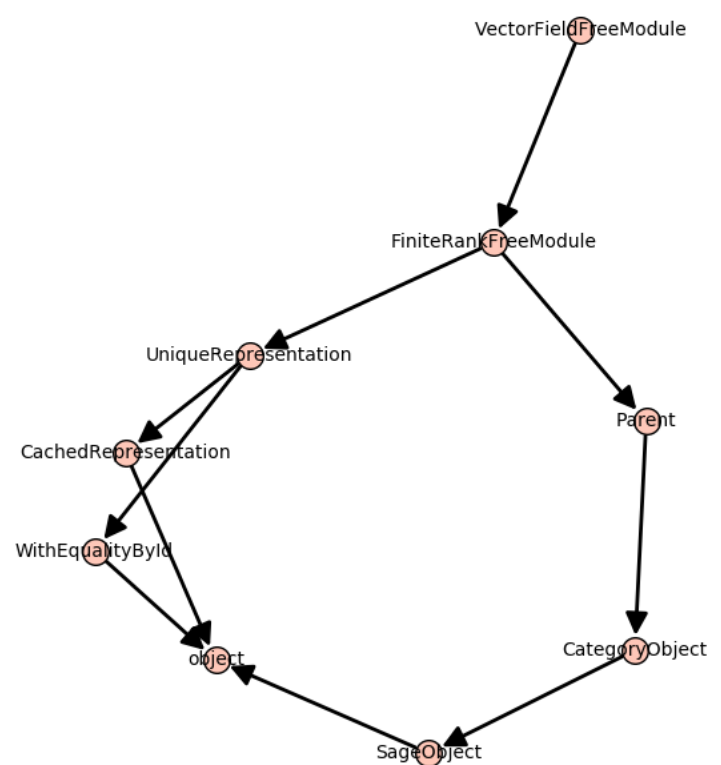
\includegraphics[width=0.7\textwidth]{vfmodule_class.png}
\caption{Output corresponding to \texttt{In [\theNBin]}.}\label{out3}
\end{figure}

Since $U$ is a chart domain, the free module $\X(U)$ is automatically endowed with a basis,
which is the coordinate frame associated to the chart:
\begin{NBin}
YU.bases()
\end{NBin}
\begin{NBoutM}
\left[\left(U, \left(\frac{\partial}{\partial x },\frac{\partial}{\partial y }\right)\right)\right]
\end{NBoutM}
Let us denote by \code{eU} this frame. We can set \code{eU = YU.bases()[0]} or
alternatively
\begin{NBin}
eU = YU.default_basis()
eU
\end{NBin}
\begin{NBoutM}
\left(U, \left(\frac{\partial}{\partial x },\frac{\partial}{\partial y }\right)\right)
\end{NBoutM}
Another equivalent instruction would have been \code{eU = U.default\_frame()}.

Similarly, $\X(V)$ is a free module, endowed with the coordinate frame
associated to stereographic coordinates from the South pole, which we
denote by \code{eV}:
\begin{NBin}
YV = V.vector_field_module()
YV.bases()
\end{NBin}
\begin{NBoutM}
\left[\left(V, \left(\frac{\partial}{\partial {x'} },\frac{\partial}{\partial {y'} }\right)\right)\right]
\end{NBoutM}
\vspace*{-\baselineskip}
\begin{NBin}
eV = YV.default_basis()
eV
\end{NBin}
\begin{NBoutM}
\left(V, \left(\frac{\partial}{\partial {x'} },\frac{\partial}{\partial {y'} }\right)\right)
\end{NBoutM}

If we consider the intersection $W=U\cap V$, we notice its module
of vector fields is endowed with two bases, reflecting the fact that
$W$ is covered by two charts: $(W,(x,y))$ and $(W,(x',y'))$:
\begin{NBin}
W = U.intersection(V)
YW = W.vector_field_module()
YW.bases()
\end{NBin}
\begin{NBoutM}
\left[\left(W, \left(\frac{\partial}{\partial x },\frac{\partial}{\partial y }\right)\right), \left(W, \left(\frac{\partial}{\partial {x'} },\frac{\partial}{\partial {y'} }\right)\right)\right]
\end{NBoutM}
Let us denote by \code{eUW} and \code{eUV} these two bases, which are
actually the restrictions of the vector frames \code{eU} and \code{eV} to
$W$:
\begin{NBin}
eUW = eU.restrict(W)
eVW = eV.restrict(W)
YW.bases() == [eUW, eVW]
\end{NBin}
\begin{NBout}
\texttt{True}
\end{NBout}
The free module $\X(W)$ is also automatically endowed with automorphisms
connecting the two bases, i.e.\ change-of-frame operators:
\begin{NBin}
W.changes_of_frame()
\end{NBin}
\begin{NBout}
\[
\bigg\{\left(\left(W, \left(\frac{\partial}{\partial {x'} },\frac{\partial}{\partial {y'} }\right)\right), \left(W, \left(\frac{\partial}{\partial x },\frac{\partial}{\partial y }\right)\right)\right) :
\]
Field of tangent-space automorphisms on the Open subset W of the 2-dimensional differentiable manifold M,
\[
\left(\left(W, \left(\frac{\partial}{\partial x },\frac{\partial}{\partial y }\right)\right), \left(W, \left(\frac{\partial}{\partial {x'} },\frac{\partial}{\partial {y'} }\right)\right)\right) :
\]
Field of tangent-space automorphisms on the Open subset W of the 2-dimensional differentiable manifold M $\bigg\}$
\end{NBout}
The first of them is
\begin{NBin}
P = W.change_of_frame(eUW, eVW)
P
\end{NBin}
\begin{NBout}
\texttt{Field of tangent-space automorphisms on the Open subset W of the 2-dimensional
differentiable manifold M}
\end{NBout}
It belongs to the general linear group of the free module $\X(W)$:
\begin{NBin}
P.parent()
\end{NBin}
\begin{NBoutM}
\mathrm{GL}\left( \mathfrak{X}\left(W\right) \right)
\end{NBoutM}
and its matrix is deduced from the Jacobian matrix of the transition map
\code{XV} $\to$ \code{XU}:
\begin{NBin}
P[:]
\end{NBin}
\begin{NBoutM}
\left(\begin{array}{rr}
-x^{2} + y^{2} & -2 \, x y \\
-2 \, x y & x^{2} - y^{2}
\end{array}\right)
\end{NBoutM}

\subsection{Construction and manipulation of vector fields}

Let us introduce a vector field $\w{v}$ on $\M$:
\begin{NBin}
v = M.vector_field(name='v')
v[eU, 0] = f.restrict(U)
v[eU, 1] = -2
v.display(eU)
\end{NBin}
\begin{NBoutM}
v = \left( \frac{1}{x^{2} + y^{2} + 1} \right) \frac{\partial}{\partial x } -2 \frac{\partial}{\partial y }
\end{NBoutM}
Notice that, at this stage, we have defined $\w{v}$ only on $U$, by setting
its components in the vector frame \code{eU}, either explicitly as scalar
fields, like the component $v^0$ set to the restriction of $f$ to $U$ or
implicitly, like the component $v^1$: the integer \code{-2}
will be coerced to the constant scalar field of value $-2$ (cf.\ Sec.~\ref{s:man:add_implement}).
We can ask for the scalar-field value of a component via the double-bracket
operator; since \code{eU} is the default frame on $M$, we do not have to specify
it:
\begin{NBin}
v[[0]]
\end{NBin}
\begin{NBoutM}
f
\end{NBoutM}
\vspace*{-\baselineskip}
\begin{NBin}
v[[0]].display()
\end{NBin}
\begin{NBoutM}
\begin{array}{llcl} f:& U & \longrightarrow & \mathbb{R} \\ & \left(x, y\right) & \longmapsto & \frac{1}{x^{2} + y^{2} + 1} \\ \mbox{on}\ W : & \left({x'}, {y'}\right) & \longmapsto & \frac{{x'}^{2} + {y'}^{2}}{{x'}^{2} + {y'}^{2} + 1} \end{array}
\end{NBoutM}
Note that, for convenience, the single bracket operator returns a chart function
of the component:
\begin{NBin}
v[0]
\end{NBin}
\begin{NBoutM}
\frac{1}{x^{2} + y^{2} + 1}
\end{NBoutM}
The restriction of $\w{v}$ to $W$ is of course
\begin{NBin}
v.restrict(W).display(eUW)
\end{NBin}
\begin{NBoutM}
v = \left( \frac{1}{x^{2} + y^{2} + 1} \right) \frac{\partial}{\partial x } -2 \frac{\partial}{\partial y }
\end{NBoutM}
Since we have a second vector frame on $W$, namely \code{eVW}, and the
change-of-frame automorphisms are known, we can ask for the components
of $\w{v}$ with respect to that frame:
\begin{NBin}
v.restrict(W).display(eVW)
\end{NBin}
\begin{NBout}
$\displaystyle
v = \left( \frac{4 \, x y^{3} - x^{2} + 4 \, {\left(x^{3} + x\right)} y + y^{2}}{x^{6} + y^{6} + {\left(3 \, x^{2} + 1\right)} y^{4} + x^{4} + {\left(3 \, x^{4} + 2 \, x^{2}\right)} y^{2}} \right) \frac{\partial}{\partial {x'} }$ \\
$\displaystyle
+ \left( -\frac{2 \, {\left(x^{4} - y^{4} + x^{2} + x y - y^{2}\right)}}{x^{6} + y^{6} + {\left(3 \, x^{2} + 1\right)} y^{4} + x^{4} + {\left(3 \, x^{4} + 2 \, x^{2}\right)} y^{2}} \right) \frac{\partial}{\partial {y'} }$
\end{NBout}
Notice that the components are expressed in terms of the coordinates $(x,y)$
since they form the default chart on $W$. To have them expressed in
terms of the coordinates $(x',y')$, we have to add the restriction of
the chart
$(V,(x',y'))$ to $W$ as the second argument of the method
\code{display()}:
\begin{NBin}
v.restrict(W).display(eVW, XV.restrict(W))
\end{NBin}
\begin{NBout}
$\displaystyle
v = \left( -\frac{{x'}^{4} - 4 \, {x'} {y'}^{3} - {y'}^{4} - 4 \, {\left({x'}^{3} + {x'}\right)} {y'}}{{x'}^{2} + {y'}^{2} + 1} \right) \frac{\partial}{\partial {x'} } $\\
$\displaystyle
+ \left( -\frac{2 \, {\left({x'}^{4} + {x'}^{3} {y'} + {x'} {y'}^{3} - {y'}^{4} + {x'}^{2} - {y'}^{2}\right)}}{{x'}^{2} + {y'}^{2} + 1} \right) \frac{\partial}{\partial {y'} }$
\end{NBout}
We extend the expression of $\w{v}$ to the full vector frame \code{XV}
by continuation of this expression:
\begin{NBin}
v.add_comp_by_continuation(eV, W, chart=XV)
\end{NBin}
\ \\
We have then
\begin{NBin}
v.display(eV)
\end{NBin}
\begin{NBout}
$\displaystyle
v = \left( -\frac{{x'}^{4} - 4 \, {x'} {y'}^{3} - {y'}^{4} - 4 \, {\left({x'}^{3} + {x'}\right)} {y'}}{{x'}^{2} + {y'}^{2} + 1} \right) \frac{\partial}{\partial {x'} }$\\
$\displaystyle
 + \left( -\frac{2 \, {\left({x'}^{4} + {x'}^{3} {y'} + {x'} {y'}^{3} - {y'}^{4} + {x'}^{2} - {y'}^{2}\right)}}{{x'}^{2} + {y'}^{2} + 1} \right) \frac{\partial}{\partial {y'} }$
\end{NBout}
At this stage, the vector field $\w{v}$ is defined in all $M$.
According to the hairy ball theorem\index{hairy ball theorem}, it has to vanish somewhere.
Let us show that this occurs at the North pole, by first introducing the
latter, as the point of stereographic coordinates $(x',y')=(0,0)$:
\begin{NBin}
N = M((0,0), chart=XV, name='N')
print(N)
\end{NBin}
\begin{NBprint}
Point N on the 2-dimensional differentiable manifold M
\end{NBprint}
As a check, we verify that the image of $N$ by the canonical embedding
$\Phi: \Sp \to \R^3$ is the point of Cartesian coordinates $(0,0,1)$:
\begin{NBin}
XR3(Phi(N))
\end{NBin}
\begin{NBoutM}
(0, 0, 1)
\end{NBoutM}
The vanishing of $\left.\w{v}\right| _N$:
\begin{NBin}
v.at(N).display()
\end{NBin}
\begin{NBoutM}
v = 0
\end{NBoutM}
On the other hand, $\w{v}$ does not vanish at the point $p$ introduced above:
\begin{NBin}
v.at(p).display()
\end{NBin}
\begin{NBoutM}
v = \frac{1}{6} \frac{\partial}{\partial x } -2 \frac{\partial}{\partial y }
\end{NBoutM}
We may plot the vector field $\w{v}$ in terms of the stereographic coordinates
from the North pole:
\begin{NBin}
v.plot(chart=XU, chart_domain=XU, max_range=2,
       number_values=5, scale=0.4, aspect_ratio=1)
\end{NBin}
\begin{center}
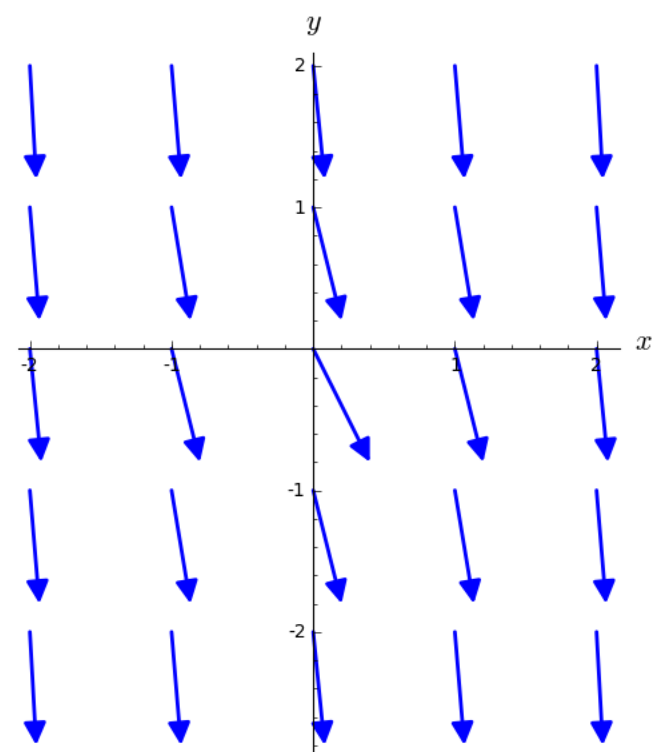
\includegraphics[width=0.6\textwidth]{plot_v_North.png}
\end{center}
or in term of those from the South pole:
\begin{NBin}
v.plot(chart=XV, chart_domain=XV, max_range=2,
       number_values=9, scale=0.05, aspect_ratio=1)
\end{NBin}
\begin{center}
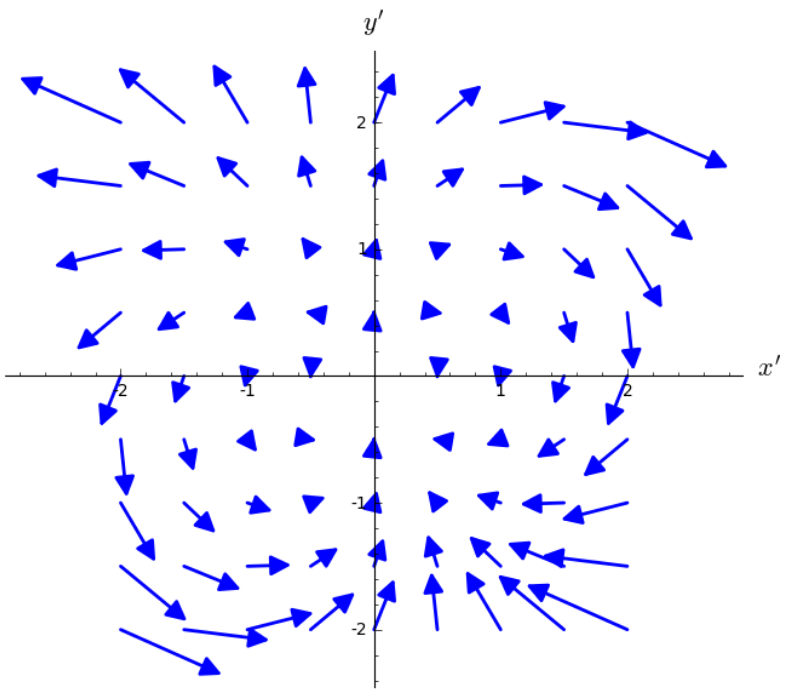
\includegraphics[width=0.8\textwidth]{plot_v_South.png}
\end{center}
Thanks to the embedding $\Phi$, we may also have a 3D plot of the vector
field $\w{v}$
atop of the 3D plot already obtained:
\begin{NBin}
graph_v = v.plot(chart=XR3, mapping=Phi, chart_domain=XU,
                 number_values=7, scale=0.2) + \
          v.plot(chart=XR3, mapping=Phi, chart_domain=XV,
                 number_values=7, scale=0.2)
show(graph + graph_v, viewer='threejs', online=True)
\end{NBin}
\begin{center}
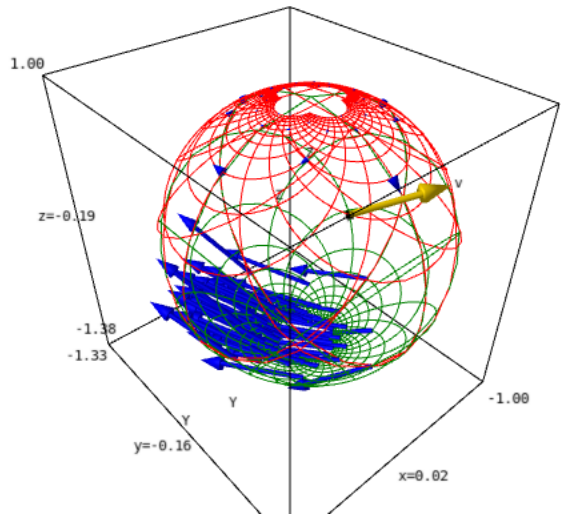
\includegraphics[width=0.6\textwidth]{plot_v_3d.png}
\end{center}
Note that the sampling, performed on the two charts \code{XU} and \code{XV}
is not uniform on the sphere. A better sampling would be achieved by introducing
spherical coordinates.

\subsection{Implementation details regarding vector fields}

Let us now investigate some internals of the implementation of vector fields.
Vector fields on $M$ are implemented via the class
\code{VectorField}\footurl{http://doc.sagemath.org/html/en/reference/manifolds/sage/manifolds/differentiable/vectorfield.html} (actually by a dynamically generated subclass of it, within \Sage{} category
framework):
\begin{NBin}
isinstance(v, sage.manifolds.differentiable.vectorfield.VectorField)
\end{NBin}
\begin{NBout}
\texttt{True}
\end{NBout}

Since $M$ is not parallelizable, the defining data of a
vector field $\w{v}$ on $M$ are its restrictions
$\left(\left. \w{v}\right| _{U_i}\right)_{1\leq i \leq m}$
to parallelizable open subsets $U_i$,
following the scheme presented in Sec.~\ref{s:vec:vector_field_impl}.
These restrictions are stored in the private dictionary \code{\_restrictions}, whose keys are
the open subsets:
\begin{NBin}
v._restrictions
\end{NBin}
\begin{NBoutM}
\left\{V : v, W : v, U : v\right\}
\end{NBoutM}
Let us consider one of these restrictions, for instance the restriction
$\left. \w{v}\right| _U$ to $U$:
\begin{NBin}
vU = v._restrictions[U]
vU is v.restrict(U)
\end{NBin}
\begin{NBout}
\texttt{True}
\end{NBout}
Since $U$ is a parallelizable open subset, the object \code{vU} belongs
to the class \code{VectorFieldParal}, which is devoted to vector fields
on parallelizable manifolds:
\begin{NBin}
isinstance(vU, sage.manifolds.differentiable.vectorfield.VectorFieldParal)
\end{NBin}
\begin{NBout}
\texttt{True}
\end{NBout}
The class \code{VectorFieldParal} inherits both from
\code{FiniteRankFreeModuleElement} (as \code{TangentVector}) and from
\code{VectorField} (see Fig.~\ref{f:vec:tensorfield_classes}).
\begin{figure}
\begin{center}
\begin{tikzpicture}[font=\small, node distance=0.5cm, minimum
height=2em, auto]

\node[native](element)
{\code{Element}};

\node[native, below=of element](module_element)
{\code{ModuleElement}};
\path[line] (module_element) -- (element);

\node[alg, below left=0.5cm and 1.5cm of module_element](freemoduletensor)
{\code{FreeModuleTensor}\\ \scriptsize {\it parent:}\\ \scriptsize
\code{TensorFreeModule}};
\path[line] (freemoduletensor) -- (module_element);

\node[alg, below=of freemoduletensor](altcontrtensor)
{\code{AlternatingContrTensor}\\ \scriptsize {\it parent:}\\ \scriptsize
\code{ExtPowerFreeModule}};
\path[line] (altcontrtensor) -- (freemoduletensor);

\node[alg, below=of altcontrtensor](finiterankfreemoduleelement)
{\code{FiniteRankFreeModuleElement}\\ \scriptsize {\it parent:}\\ \scriptsize
\code{FiniteRankFreeModule}};
\path[line] (finiterankfreemoduleelement) -- (altcontrtensor);

\node[diff, below=of finiterankfreemoduleelement](tangentvector)
{\code{TangentVector}\\ \scriptsize {\it parent:}\\ \scriptsize
\code{TangentSpace}};
\path[line] (tangentvector) -- (finiterankfreemoduleelement);


\node[diff, right=6cm of freemoduletensor](tensorfield)
{\code{TensorField}\\ \scriptsize {\it parent:}\\ \scriptsize
\code{TensorFieldModule}};
\path[line] (tensorfield) -- (module_element);

\node[diff, below=of tensorfield](multivectorfield)
{\code{MultivectorField}\\ \scriptsize {\it parent:}\\ \scriptsize
\code{MultivectorModule}};
\path[line] (multivectorfield) -- (tensorfield);

\node[diff, below=of multivectorfield](vectorfield)
{\code{VectorField}\\ \scriptsize {\it parent:}\\ \scriptsize
\code{VectorFieldModule}};
\path[line] (vectorfield) -- (multivectorfield);

\node[diff, right=1.2cm of altcontrtensor](tensorfieldparal)
{\code{TensorFieldParal}\\ \scriptsize {\it parent:}\\ \scriptsize
\code{TensorFieldFreeModule}};
\path[line] (tensorfieldparal) -- (freemoduletensor);
\path[line] (tensorfieldparal) -- (tensorfield);

\node[diff, below=of tensorfieldparal](multivectorfieldparal)
{\code{MultivectorFieldParal}\\ \scriptsize {\it parent:}\\ \scriptsize
\code{MultivectorFreeModule}};
\path[line] (multivectorfieldparal) -- (altcontrtensor);
\path[line] (multivectorfieldparal) -- (tensorfieldparal);

\node[diff, below=of multivectorfieldparal](Vectorfieldparal)
{\code{VectorFieldParal}\\ \scriptsize {\it parent:}\\ \scriptsize
\code{VectorFieldFreeModule}};
\path[line] (Vectorfieldparal) -- (finiterankfreemoduleelement);
\path[line] (Vectorfieldparal) -- (multivectorfieldparal);
\path[line] (Vectorfieldparal) -- (vectorfield);


% legend
\node[native_legend, below left=0.4cm and -0.5cm of vectorfield]
(native_legend){};
\node[empty, right=0.5em of native_legend]
{Generic \Sage{} class};

\node[alg_legend, below=1.em of native_legend]
(alg_legend){};
\node[empty, right=0.5em of alg_legend]
{\SM{} class\\ \footnotesize (algebraic part)};

\node[diff_legend, below=1.5em of alg_legend]
(diff_legend){};
\node[empty, right=0.5em of diff_legend]
{\SM{} class\\ \footnotesize (differential part)};

\end{tikzpicture}

\end{center}
\caption{\label{f:vec:tensorfield_classes}\footnotesize
\Sage{} classes for tensor fields involved in differentiable manifolds.
There are various multiple inheritances involving diamond diagrams;
Python's method resolution order algorithm (MRO) relies on the ordering of the parents
in the class declaration and this order can be read from the left to the right in
this figure. For instance, the class \code{VectorFieldParal} is declared as
\code{class VectorFieldParal(FiniteRankFreeModuleElement, MultivectorFieldParal, VectorField)}.}
\end{figure}
The defining data of $\left. \w{v}\right| _U$ are
its sets of components with respect to (possibly various)
vector frames on $U$, according to Eq.~\eqref{e:vec:vi_expand}. The sets of components are stored in the private dictionary \code{\_components}, whose keys are the vector frames:
\begin{NBin}
vU._components
\end{NBin}
\begin{NBoutM}
\left\{\left(U, \left(\frac{\partial}{\partial x },\frac{\partial}{\partial y }\right)\right) :
\mbox{\texttt{1-index components w.r.t.~Coordinate frame (U, (d/dx,d/dy))}}\right\}
\end{NBoutM}
Similarly, we have:
\begin{NBin}
v._restrictions[W]._components
\end{NBin}
\begin{NBout}
\[
\bigg\{\left(W, \left(\frac{\partial}{\partial x },\frac{\partial}{\partial y }\right)\right) :
\mbox{\texttt{1-index components w.r.t.~Coordinate frame (W, (d/dx,d/dy))}},
\]
\[
\left(W, \left(\frac{\partial}{\partial {x'} },\frac{\partial}{\partial {y'} }\right)\right) :
\mbox{\texttt{1-index components w.r.t.~Coordinate frame (W, (d/dxp,d/dyp)}}
\bigg\}
\]
\end{NBout}
The values of the dictionary \code{\_components} belong to the same class
\code{Components} as that discussed in Sec.~\ref{s:vec:tangent_impl} for
the storage of components of tangent vectors:
\begin{NBin}
vUc = vU._components[eU]
vUc
\end{NBin}
\begin{NBout}
\texttt{1-index components w.r.t.~Coordinate frame (U, (d/dx,d/dy))}
\end{NBout}
\vspace*{-\baselineskip}
\begin{NBin}
type(vUc)
\end{NBin}
\begin{NBout}
\begin{verbatim}
<class 'sage.tensor.modules.comp.Components'>
\end{verbatim}
\end{NBout}
As already mentioned in Sec.~\ref{s:vec:tangent_impl}, the components themselves are stored
in the private attribute \code{\_comp} of the \code{Components} object; this is a dictionary
whose keys are the indices:
\begin{NBin}
vUc._comp
\end{NBin}
\begin{NBout}
$\displaystyle
\big\{\left(0\right) : f, $\\
$\displaystyle
\phantom{x}\left(1\right) : \mbox{Scalar field on the Open subset U of the 2-dimensional differentiable manifold M}\big\}$
\end{NBout}
The difference with the tangent vector case is that the values of that dictionary are now scalar fields, i.e.\ elements of $C^\infty(U)$ in the present case. This is of course in agreement with the treatment of $\mathfrak{X}(U)$ as a free module over $C^\infty(U)$,
as discussed in Sec.~\ref{s:vec:vector_field_impl}.
Taking into account the storage of scalar fields presented in Sec.~\ref{s:man:def_scalar},
the full storage structure of vector fields is presented in Fig.~\ref{f:vec:storage_tensor}
(the latter actually regards tensor fields, of which vector fields constitute a subcase).

\begin{figure}
\begin{center}
\begin{tikzpicture}[font=\footnotesize, remember picture,
node distance=0.5em, minimum height=0.5em, auto]

\node[tens, align=center](tensorfield)
{\code{TensorField}\\ \normalsize $T$};

% Restrictions
\node[dict, below=of tensorfield](restrictions){
\begin{tikzpicture}
  \node[empty, align=left](description)
  {\bf dictionary \textcolor{red}{\code{TensorField.\_restrictions}}};
  \node[empty, below left=of description](domain1)
  {domain 1:\\ {\normalsize $U_1$}};
  \node[tens, right=0em of domain1](tensorfield1)
  {\code{TensorFieldParal}\\
  {\normalsize $T|_{U_1}=T^a_{\ \, b} e_a\otimes
e^b=T^{\hat{a}}_{\ \, \hat{b}}\varepsilon_{\hat{a}}\otimes
\varepsilon^{\hat{b}}=\dots$}};
  \node[empty, right=of tensorfield1](domain2)
  {domain 2:\\ {\normalsize $U_2$}};
  \node[tens, align=center, right=0em of domain2](tensorfield2)
  {\code{TensorFieldParal}\\ {\normalsize $T|_{U_2}$}};
  \node[empty, right=of tensorfield2](more)
  {\large $\dots$};
\end{tikzpicture}
};

% Components
\node[dict, below=of restrictions](components){
\begin{tikzpicture}
  \node[empty, align=left](description)
  {\bf dictionary
\textcolor{red}{\code{TensorFieldParal.\_components}}};
  \node[empty, below left=of description](frame1)
  {frame 1:\\ {\normalsize $(e_a)$}};
  \node[tens, right=0em of frame1](components1)
  {\code{Components}\\
  {\normalsize $(T^a_{\ \, b})_{1\le a,\,b\,\le n}$}};
  \node[empty, right=of components1](frame2)
  {frame 2:\\ {\normalsize $(\varepsilon_{\hat{a}})$}};
  \node[tens, right=0em of frame2](components2)
  {\code{Components}\\
  {\normalsize $(T^{\hat{a}}_{\ \, \hat{b}})_{1\le
\hat{a},\,\hat{b}\,\le n}$}};
  \node[empty, right=of components2](more)
  {\large $\dots$};
\end{tikzpicture}
};

% comp Scalarfields
\node[dict, below=of components](comp){
\begin{tikzpicture}
  \node[empty, align=left](description)
  {\bf dictionary \textcolor{red}{\code{Components.\_comp}}};
  \node[empty, below left=of description](comp1)
  {\normalsize $(1,1):$};
  \node[tens, align=center, right=0em of comp1](scalarfield1)
  {\code{DiffScalarField}\\
  {\normalsize $T^1_{\ \, 1}$}};
  \node[empty, right=of scalarfield1](comp2)
  {\normalsize $(1,2):$};
  \node[tens, align=center, right=0em of comp2](scalarfield2)
  {\code{DiffScalarField}\\
  {\normalsize $T^1_{\ \, 2}$}};
  \node[empty, right=of scalarfield2](more)
  {\large $\dots$};
\end{tikzpicture}
};

% Scalarfield express
\node[dict, below=of comp](express){
\begin{tikzpicture}
  \node[empty, align=left](description)
  {\bf dictionary \textcolor{red}{\code{DiffScalarField.\_express}}};
  \node[empty, below left=of description](chart1)
  {chart 1:\\
  {\normalsize $\left(x^a\right)$}};
  \node[tens, right=0em of chart1](functionchart1)
  {\code{ChartFunction}\\
  {\normalsize $T^1_{\ \, 1}\left(x^1,\dots,x^n\right)$}};
  \node[empty, right=of functionchart1](chart2)
  {chart 2:\\
  {\normalsize $\left(y^a\right)$}};
  \node[tens, right=0em of chart2](functionchart2)
  {\code{ChartFunction}\\
  {\normalsize $T^1_{\ \, 1}\left(y^1,\dots,y^n\right)$}};
  \node[empty, right=of functionchart2](more)
  {\large $\dots$};
\end{tikzpicture}
};

% expressions
\node[dict, below=0.3cm of functionchart1](chartfexpress){
\begin{tikzpicture}
  \node[empty, align=left](description)
  {\bf dictionary \textcolor{red}{\code{ChartFunction.\_express}}};
  \node[empty, below left=of description](methSR)
  {SR:};
  \node[tens, right=0em of methSR](exprSR)
  {\code{Expression}\\
  {\normalsize $x^1\cos x^2$}};
  \node[empty, right=of exprSR](methSymPy)
  {SymPy:};
  \node[tens, right=0em of methSymPy](exprSymPy)
  {\code{Basic}\\
  {\normalsize $x^1\cos x^2$}};
  \node[empty, right=of exprSymPy](more)
  {\large $\dots$};
\end{tikzpicture}
};


% lines
\draw[thick, line width=0.2em, black!60,-] (restrictions) -- (tensorfield);
\draw[thick, line width=0.2em, black!60,-] (components) -- (tensorfield1);
\draw[thick, line width=0.2em, black!60,-] (comp) -- (components1);
\draw[thick, line width=0.2em, black!60,-] (express) -- (scalarfield1);
\draw[thick, line width=0.2em, black!60,-] (chartfexpress) -- (functionchart1);

\end{tikzpicture}

\end{center}
\caption{\label{f:vec:storage_tensor} \footnotesize
Internal storage of tensor fields. Red boxes
represent Python dictionaries, yellow boxes are dictionary values, with the corresponding
dictionary key located on the left of them.
The Python class of each dictionary value is indicated in typewriter font at the top of the
yellow box. In the hierarchical tree, only the leftmost
branch is indicated by grey connectors. In the special case of vector fields, the classes
\code{TensorField} and \code{TensorFieldParal} are to be replaced by \code{VectorField} and \code{VectorFieldParal} respectively.}
\end{figure}

Let us perform some algebraic operation on vector fields:
\begin{NBin}
w = v + f*v
w
\end{NBin}
\begin{NBout}
Vector field on the 2-dimensional differentiable manifold M
\end{NBout}
The code for the addition is accessible via
\begin{NBin}
v.__add__??
\end{NBin}
\begin{lstlisting}
File: .../src/sage/structure/element.pyx
def __add__(left, right):
    """
    Top-level addition operator for :class:`Element` invoking
    the coercion model.

    See :ref:`element_arithmetic`.
    ...
    """
    cdef int cl = classify_elements(left, right)
    if HAVE_SAME_PARENT(cl):
        return (<Element>left)._add_(right)
    # Left and right are Sage elements => use coercion model
    if BOTH_ARE_ELEMENT(cl):
        return coercion_model.bin_op(left, right, add)
    ...
\end{lstlisting}
This is exactly the same method \code{\_\_add\_\_()} as that discussed in
Sec.~\ref{s:man:add_implement} for the addition of scalar fields (cf.\ page~\pageref{p:man:list___add__}), namely
the method \code{\_\_add\_\_()} of the top-level class \code{Element}, from
which both \code{VectorField} and \code{DiffScalarField} inherit, cf.\ the inheritance
diagrams of Figs.~\ref{f:vec:tensorfield_classes} and
\ref{f:man:scalar_classes} (taking into account that
\code{CommutativeAlgebraElement} is a subclass of \code{Element}).
In the present case, \code{left} = \code{v} and \code{right} = \code{f*v}
have the same parent, so that the actual result is computed in line~12,
via the method \code{\_add\_()}
(note the single underscore on each side of \code{add}). This operator is
implemented at the level of \code{TensorField}, as it can be checked from the source code
(see lines~3 and 29 below):
\begin{NBin}
v._add_??
\end{NBin}
\begin{lstlisting}
def _add_(self, other):
    """
    Tensor field addition.

    INPUT:

    - ``other`` -- a tensor field, in the same tensor module as ``self``

    OUTPUT:

    - the tensor field resulting from the addition of ``self``
      and ``other``
    ...
    """
    resu_rst = {}
    for dom in self._common_subdomains(other):
        resu_rst[dom] = self._restrictions[dom] + other._restrictions[dom]
    some_rst = next(itervalues(resu_rst))
    resu_sym = some_rst._sym
    resu_antisym = some_rst._antisym
    resu = self._vmodule.tensor(self._tensor_type, sym=resu_sym,
                                antisym=resu_antisym)
    resu._restrictions = resu_rst
    if self._name is not None and other._name is not None:
        resu._name = self._name + '+' + other._name
    if self._latex_name is not None and other._latex_name is not None:
        resu._latex_name = self._latex_name + '+' + other._latex_name
    return resu
File:  .../site-packages/sage/manifolds/differentiable/tensorfield.py
\end{lstlisting}
The first step in the addition of two vector fields is to search in the
restrictions of both vector fields for common domains: this is performed in
line~16, via the method \code{\_common\_subdomains}. Then the addition is
performed at the level of the restrictions, in line~17. The rest of the code
is simply the set up of the vector field object containing the result.
Recursively, the addition performed in line~17 will reach a level at which
the domains are parallelizable. Then a different method \code{\_add\_()}, will
be involved, as we can check on \code{vU}:
\begin{NBin}
vU._add_??
\end{NBin}
\begin{lstlisting}
def _add_(self, other):
    """
    Tensor addition.

    INPUT:

    - ``other`` -- a tensor, of the same type as ``self``

    OUTPUT:

    - the tensor resulting from the addition of ``self`` and ``other``
    ...
    """
    # No need for consistency check since self and other are guaranted
    # to belong to the same tensor module
    basis = self.common_basis(other)
    if basis is None:
        raise ValueError("no common basis for the addition")
    comp_result = self._components[basis] + other._components[basis]
    result = self._fmodule.tensor_from_comp(self._tensor_type, comp_result)
    if self._name is not None and other._name is not None:
        result._name = self._name + '+' + other._name
    if self._latex_name is not None and other._latex_name is not None:
        result._latex_name = self._latex_name + '+' + other._latex_name
    return result
File:   .../site-packages/sage/tensor/modules/free_module_tensor.py
\end{lstlisting}
From line~26, we see that this method \code{\_add\_()} is implemented
at the level of tensors on free modules, i.e.\ in the class
\code{FreeModuleTensor},\footurl{http://doc.sagemath.org/html/en/reference/tensor_free_modules/sage/tensor/modules/free_module_tensor.html}
from which \code{VectorFieldParal} inherits (cf.\ the diagram in
Fig.~\ref{f:vec:tensorfield_classes}). Here the free module is clearly
$\mathfrak{X}(U)$. The addition amounts to adding the components in a
basis of the free module in which both operands have known components. Such
a basis is returned by the method \code{common\_basis} invoked in line~16.
If necessary, this method can use change-of-basis formulas to compute the
components of \code{self} or \code{other} in a common basis.
The addition of the components in the found basis is performed in line~19. It
involves the method \code{\_\_add\_\_()} of class \code{Components}; we
can examine the corresponding code via the object \code{vUc} since the
latter has been defined above as \code{vUc = vU.\_components[eU]}, i.e.
\code{vUc} represents the set of components of the vector field
$\left. \w{v}\right| _U$ in the basis \code{eU} $=(\partial/\partial x, \partial/\partial y)$
of $\mathfrak{X}(U)$:
\begin{NBin}
vUc.__add__??
\end{NBin}
\begin{lstlisting}
def __add__(self, other):
    """
    Component addition.

    INPUT:

    - ``other`` -- components of the same number of indices and defined
      on the same frame as ``self``

    OUTPUT:

    - components resulting from the addition of ``self`` and ``other``
    ...
    """
    ...
    result = self.copy()
    nproc = Parallelism().get('tensor')
    if nproc != 1 :
        # Parallel computation
        ...
    else:
        # Sequential computation
        for ind, val in other._comp.items():
            result[[ind]] += val
    return result
File:   .../site-packages/sage/tensor/modules/comp.py
\end{lstlisting}
First of all, we note from line~26
that this is not the method \code{\_\_add\_\_()} of class \code{Element},
as it was for \code{VectorField} and \code{VectorFieldParal},
but instead the method \code{\_\_add\_\_()} implemented
in class \code{Components}. This is because \code{Components} is a
\emph{technical} class, as opposed to the \emph{mathematical} classes
\code{VectorField} and \code{DiffScalarField}; therefore it does not
inherits from \code{Element}, but only from the base class \code{SageObject},
which does not implement any addition.
We note from lines~17-19
that the computation of the components can be done in parallel on more that one CPU core if user has turned on parallelization.\footnote{This is done with the command
\code{Parallelism().set(nproc=8)} (for 8 threads); many examples of
parallelized computations are presented at
\url{https://sagemanifolds.obspm.fr/examples.html}.}
Focusing on the sequential code (lines~23-24), we see that the addition is
performed component by component.
Note that this addition is that
of scalar fields, as discussed in Sec.~\ref{s:man:add_implement},
since each component being an element of $C^\infty(U)$, the base ring of $\mathfrak{X}(U)$.

\subsection{Action of vector fields on scalar fields} \label{s:vec:action_on_scalar}

The action of $\w{v}$ on $f$ is defined pointwise by
considering $\w{v}$ at each point $p\in M$ as a derivation (the very definition of a tangent vector,
cf.\ Sec.~\ref{s:vec:def_tangent_vector}); the result is then a scalar field $\w{v}(f)$ on $M$:
\begin{NBin}
vf = v(f)
vf
\end{NBin}
\begin{NBoutM}
v\left(f\right)
\end{NBoutM}
\vspace*{-\baselineskip}
\begin{NBin}
vf.display()
\end{NBin}
\begin{NBoutM}
\begin{array}{llcl} v\left(f\right):& M & \longrightarrow & \mathbb{R} \\ \mbox{on}\ U : & \left(x, y\right) & \longmapsto & \frac{2 \, {\left(2 \, y^{3} + 2 \, {\left(x^{2} + 1\right)} y - x\right)}}{x^{6} + y^{6} + 3 \, {\left(x^{2} + 1\right)} y^{4} + 3 \, x^{4} + 3 \, {\left(x^{4} + 2 \, x^{2} + 1\right)} y^{2} + 3 \, x^{2} + 1} \\[1ex] \mbox{on}\ V : & \left({x'}, {y'}\right) & \longmapsto & -\frac{2 \, {\left({x'}^{5} + 2 \, {x'}^{3} {y'}^{2} + {x'} {y'}^{4} - 2 \, {y'}^{5} - 2 \, {\left(2 \, {x'}^{2} + 1\right)} {y'}^{3} - 2 \, {\left({x'}^{4} + {x'}^{2}\right)} {y'}\right)}}{{x'}^{6} + {y'}^{6} + 3 \, {\left({x'}^{2} + 1\right)} {y'}^{4} + 3 \, {x'}^{4} + 3 \, {\left({x'}^{4} + 2 \, {x'}^{2} + 1\right)} {y'}^{2} + 3 \, {x'}^{2} + 1} \end{array}
\end{NBoutM}
